  \documentclass[11pt, oneside]{article}   	% use "amsart" instead of "article" for AMSLaTeX format
\usepackage{geometry}                		% See geometry.pdf to learn the layout options. There are lots.
\geometry{letterpaper}                   		% ... or a4paper or a5paper or ... 
%\geometry{landscape}                		% Activate for for rotated page geometry
%\usepackage[parfill]{parskip}    		% Activate to begin paragraphs with an empty line rather than an indent
\usepackage{graphicx}				% Use pdf, png, jpg, or eps§ with pdflatex; use eps in DVI mode
								% TeX will automatically convert eps --> pdf in pdflatex		
\usepackage{amssymb}
\usepackage{amsmath}
\usepackage{parskip}
\usepackage{color}
\usepackage{hyperref}

\title{Partial fractions}
%\author{The Author}
%\section{}
%\subsection*{}
\date{}							% Activate to display a given date or no date

\graphicspath{{/Users/telliott_admin/Dropbox/Tex/png/}}
% \begin{center} 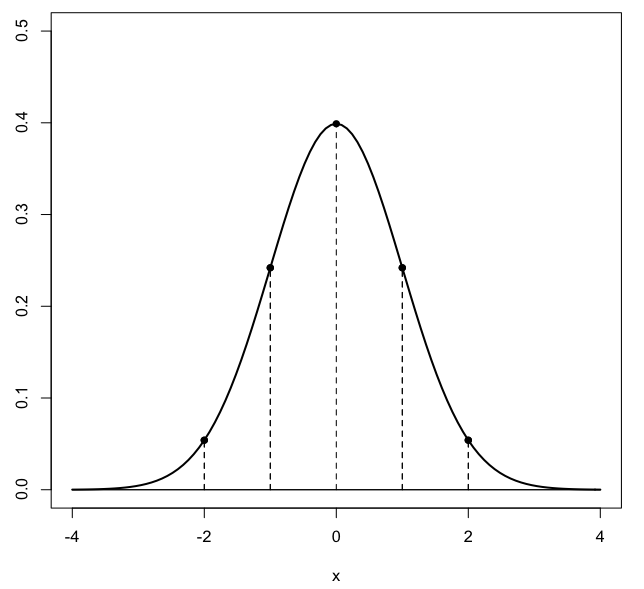
\includegraphics [scale=0.4] {gauss3.png} \end{center}
\begin{document}
\maketitle
\Large
In the previous section, we derived Cauchy 2
\[ \oint_C \frac{f(z)}{z-z_0} \ dz = 2 \pi i f(z_0) \]
One example is
\[ \oint_C \frac{1}{z-z_0} \ dz = 2 \pi i \]
which is easy to show even without using the new formula.

\subsection*{Example 1}
This problem is Beck 4.26.  Consider 
\[ \oint f(z) \ dz = \oint \frac{1}{z^2 + 1} \ dz \]
We see that the denominator is zero when
\[ z^2 = -1 \]
\[ z = \pm \ i \]
Therefore we can factor the denominator as
\[ z^2 + 1 = (z + i) (z-i) \]

There are a couple of different ways to handle this.  One is to use partial fractions:
\[ \frac{1}{z^2 + 1} = \frac{1}{(z + i) (z-i)} \]
\[ = \frac{1}{2i} \ [ \ \frac{1}{z - i} - \frac{1}{z+i} \ ] \]
So the integral is a sum of two integrals:
\[ I = \frac{1}{2i} \ [ \oint \frac{1}{z - i}  \ dz -  \oint \frac{1}{z + i} \ dz \ ] \] 

Suppose the curve is the unit circle centered at $i$, designated as $C[i,1]$.  Obviously, this curve contains the singularity $z = i$.  The curve goes through the origin, so it does not extend as far as $z = -i$.

Therefore, the second integral is zero (no singularity) and the first is
\[ \frac{1}{2i} \ [ \ \oint \frac{1}{z - i}  \ dz \ ] \ = \frac{1}{2i} \ [ \  2 \pi i \ ] \]
by Cauchy 2.  Thus the value is just $I = \pi$

According to Beck, as an alternative, rewrite the function as
\[ \frac{1}{(z + i) (z-i)} = \frac{(1/z+i)}{z-i} \]
Thus
\[ \int \frac{1}{z^2 + 1} \ dz = \int \frac{(1/z+i)}{z-i} \ dz \]
We have essentially the same thing.  The function is
\[ \frac{1}{z+i} \]
and when evaluated at $i$, with result $1/2i$, we obtain
\[ \oint  \frac{f(z)}{z-z_0} \ dz = 2 \pi i \ f(z_0) \]
\[ = 2 \pi i \ \frac{1}{2i} = \pi \]

\subsection*{partial fractions}
We can also do the curve containing both singularities by using the formal apparatus of partial fractions.  Write
\[ \frac{1}{z^2 + 1} = \frac{1}{(z+i)(z-i)} \]
\[ = \frac{A}{z+i} + \frac{B}{z-i} \]
We need to determine $A$ and $B$.  When we multiply to put everything over the common denominator ($z^2 + 1)$ then for the numerators we will have:
\[ A(z-i) + B(z+i) = 1 \]
All the powers of $z$ must match across the equal sign.  So this gives
\[ -Ai + Bi = 1 \]
\[ Az + Bz = 0 \]
From the second we get that $A = -B$.  And so from the first
\[ -Ai - Ai = -2Ai = 1 \]
\[ A = -\frac{1}{2i} \]
Hence the integrand is
\[ \frac{1}{z^2 + 1} = = \frac{A}{z+i} + \frac{B}{z-i} \]
\[ = -\frac{1}{2i(z+i)} + \frac{1}{2i(z-i)} \]
which matches what we had above:
\[ = \frac{1}{2i} \ [ \ \frac{1}{z - i} - \frac{1}{z+i} \ ] \]

For the curve including $z = i$ but not $z = -i$ we have that the left-hand integral is 0 by Cauchy's Theorem, and for the right hand side the function is
\[ f(z = z_0) = \frac{1}{2i} \]
So the value of the integral is
\[ 2 \pi i f(z_0) = 2 \pi i \ \frac{1}{2i} = \pi \]
as before.  The other pole we would have
\[ f(z = z_0) = -\frac{1}{2i} \]
and the result would be $- \pi$.  A curve enclosing both poles would have integral equal to zero.

\subsection*{example}
Consider
\[ \int_{\gamma} \frac{z^2}{4-z^2} \ dz \]
where $\gamma = | z + 1 | = 2$.
So the denominator of the function is
\[ \frac{1}{4-z^2} = \frac{1}{(2+z)(2-z)} \]
It has zeroes as $z = \pm \ 2$.  Only the point $z = 2$ is inside our contour.  So if we split this by partial fractions
\[  \frac{1}{(2+z)(2-z)} = \frac{1}{4} \ [ \ \frac{1}{2+z} + \frac{1}{2-z} \ ] \]
so we can rewrite the integral as
\[ I = \int_{\gamma} \frac{z^2}{4} \ [ \ \frac{1}{2+z} + \frac{1}{2-z} \ ] \ dz \]

By Cauchy's Theorem, the first term is zero.  The second one is:
\[ I = \int_{\gamma} \frac{z^2}{4} \ ( \frac{1}{2-z} ) \ dz \]
and the value of $I$ is
\[ I = 2 \pi i f(z_0) \]
where 
\[ f(z_0) = \frac{z^2}{4}  \ \bigg |_{z_0 = 2} = 1 \]
so the integral is just $2 \pi i$.

\subsection*{one from wikipedia}
Consider
\[ g(z) = \frac{z^2}{z^2 + 2z + 2} \]
We want to evaluate the integral:
\[ I = \oint g(z) \ dz \]

The denominator
\[ z^2 + 2z + 2 \]
can be factored.

We plug into the quadratic solution:
\[ \frac{-b \pm \sqrt{b^2 - 4ac}}{2a} =  \frac{-2 \pm \sqrt{4 - 4 \cdot 2}}{2} \]
\[ = -1 \pm \  \frac{\sqrt{-4}}{2} \]
\[ = -1 \pm i \]
The zeroes of the denominator are
\[ - 1 + i \ , \ \ \ - 1 - i \]
From this we construct the two factors as
\[ z - (- 1 + i) = z + 1 - i \]
\[ z - (-1 - i) = z + 1 + i \]

We confirm that these two factors multiplied together give back what we started with:
\[ (z + 1 + i) \ (z + 1 - i) \]
\[ = z^2 + z + iz + z + 1 + i + -iz - i + 1 \] 
\[ = z^2 + 2z + 2 \]

So we can factor the denominator and write:
\[ \frac{1}{z^2 + 2z + 2} = \frac{A}{z + 1 - i} + \frac{B}{z + 1 + i}  \]
Putting these two terms over a common denominator means multiplying the two factors and restoring what we started with.

For the numerator we have
\[ A(z + 1 + i) + B(z + 1 - i) = 1 \]
\[ Az + A + iA + Bz + B - iB = 1 \]
Equating terms containing the same power of $z$ gives two simultaneous equations:
\[ Az + Bz = 0z \]
and
\[ A(1 + i) + B(1 - i) = 1 \]

So $A = -B$ and
\[ A(1 + i) + B(1 - i) = 1 \]
\[ A (1 + i) - A(1 - i) = 1 \]
\[ A 2i = 1 \]
\[ A = \frac{1}{2i}, \ \ \ B = -\frac{1}{2i} \]
The integral is
\[ \oint \frac{z^2}{2i} \ [ \ \ \frac{1}{z + (1 - i)} -  \frac{1}{z + (1 + i)} \ ] \ dz \]

So we see that we have a sum of integrals of the form
\[ \oint \frac{f(z)}{z - z_0} \]
The residues occur at the points
\[ z = z_0 \]
that is at 
\[ z = - (1 - i) = -1 + i \]
\[ z = - (1 + i) = -1 - i \]

If the contour is $|z| = 2$ centered at the origin (the circle of radius $2$, then both of the points lie within the contour.  ($ r^2 = 2$ for both).

We evaluate $2 \pi i f(z_0)$ for each
\[ f(z) = \frac{z^2}{2i} \]
The first term gives
\[ f(z_0) = \frac{(-1 + i)^2}{2i} =  \frac{1 - 1 - 2i}{2i} = -1 \]
The second term gives 
\[ \frac{(-1 -i)^2}{2i} = \frac{-1 - 1 + 2i}{2i} = 1 \]
But...  this is not quite right.  Go back and see that the second term in the integral has a minus sign.  Hence the result at this step is $-1$ for both.

Each of these needs to be multiplied by $2 \pi i$ and then summed.
\[ I = -4 \pi i \]

\end{document}  
